\documentclass[a4paper,10pt]{report}
\usepackage[utf8]{inputenc}
\usepackage{amssymb}
\usepackage{amsthm}
\usepackage{amsmath}
\usepackage{graphicx}
\usepackage[bookmarksopen, linktocpage]{hyperref}
\setlength{\parindent}{0pt}

\newcommand{\norm}[1]{\lVert#1\rVert} 		%Double vertical bars for norms
\newcommand{\ip}[2]{\langle#1,#2\rangle}	%Inner product
\newcommand{\vb}[1]{\mathbf{#1}}		%Bold vector

\makeatletter
\renewcommand*\env@matrix[1][*\c@MaxMatrixCols c]{%
  \hskip -\arraycolsep
  \let\@ifnextchar\new@ifnextchar
  \array{#1}}
\makeatother
% Augmented matrices. Use like this:
% \begin{pmatrix}[cc|c]

\begin{document}
\title{Circuits, Spring 2014 Notes}
\author{Zack Garza}
\maketitle
\tableofcontents

\chapter{LRC}
\section{Inductors}
Current can not change instantaneously.
Can be combined like resistors.

\begin{figure}[htpb]
	\begin{centering}
	\begin{center}
	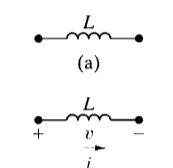
\includegraphics{./inductor_sign_convention.png}
	\caption{Inductor Sign Conventions}
	\label{fig:inductor_sign_convention}
	\end{center}
	\par\end{centering}
\end{figure}

\begin{align*}
	v &= L \frac{di}{dt} \\
	i{t} &= \frac{1}{L} \int_0^t v dt + i(t_0)
\end{align*}

Power in an inductor:
\begin{align*}
	p = Li\frac{di}{dt}
\end{align*}

Energy in an inductor:
\begin{align*}
	w &= \frac{1}{2}Li^2
\end{align*}


\section{Capacitors}
Voltage can not change instantaneously.
\begin{figure}[htpb]
	\begin{centering}
	\begin{center}
	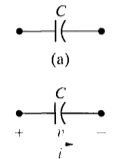
\includegraphics{./capacitor_sign_convention.png}
	\caption{Capacitor Sign Conventions}
	\label{fig:capacitor_sign_convention}
	\end{center}
	\par\end{centering}
\end{figure}

\begin{align*}
	i &= C\frac{dv}{dt} \\
	v(t) &= \frac{1}{C}\int_{t_0}^t i dt + v(t_0) \\
	p &= Cv\frac{dv}{dt} \\
	w &= \frac{1}{2}Cv^2
\end{align*}


\end{document}